\documentclass[a4paper, 12pt]{article}
\usepackage{graphicx}
\usepackage[a4paper, top=2cm , bottom=2cm , right=2cm , left=2cm ]{geometry}
\usepackage{graphicx} % Required for inserting images
\usepackage[T1]{fontenc}
\usepackage[latin1]{inputenc}
\usepackage{glossaries}
\usepackage{graphicx}
\usepackage{amsfonts}
\usepackage[hidelinks]{hyperref}
\usepackage{pifont}
\usepackage{eufrak}
\usepackage{float}
\usepackage{verbatim}
\usepackage{amssymb}
\usepackage{listings}
\usepackage{amsthm}
\usepackage{matlab-prettifier}
\usepackage{pifont}
\usepackage{multicol}
\usepackage{verbatim}
\usepackage{tikz}
\usetikzlibrary{shapes,arrows}
\usepackage{tikz}
\tikzstyle{mybox} = [draw=black, thin, rectangle, rounded corners, inner ysep=5pt, inner xsep=5pt, fill=blue!15]
\newtheorem{theorem}{Theorem}

\usepackage[affil-it]{authblk}
\usepackage{cleveref}
\usepackage{booktabs} % To thicken table lines

\title{\textbf{Structured uncertainty and $\mu$-analysis}}


\author{Carlo Migliaccio
%\\Master's Degree in Computer Engineering\\
%Politecnico di Torino}
}
\date{December 2024}

\begin{document}
\maketitle

\section{Structured uncertainty}
Dealing with \textbf{structured uncertainty} and the analysis of feedback control systems affected by it we are going to consider the \textit{general control configuration} depicted in the figure below.
Here $z_\Delta$ and $w_\Delta$ are the so-called \textit{uncertainty channels}, which in turn are the signals connecting the \textbf{uncertainty sources} with the known part of the feedback system. On the other hand the signals $z_p$ and $w_p$ are chosen in order to satisfy \textbf{performance requirements} from which the name \textbf{performance channel}. In the following we deal with mainly with \textbf{parametric uncertainty}.


\begin{multicols}{2}
    \begin{center}
        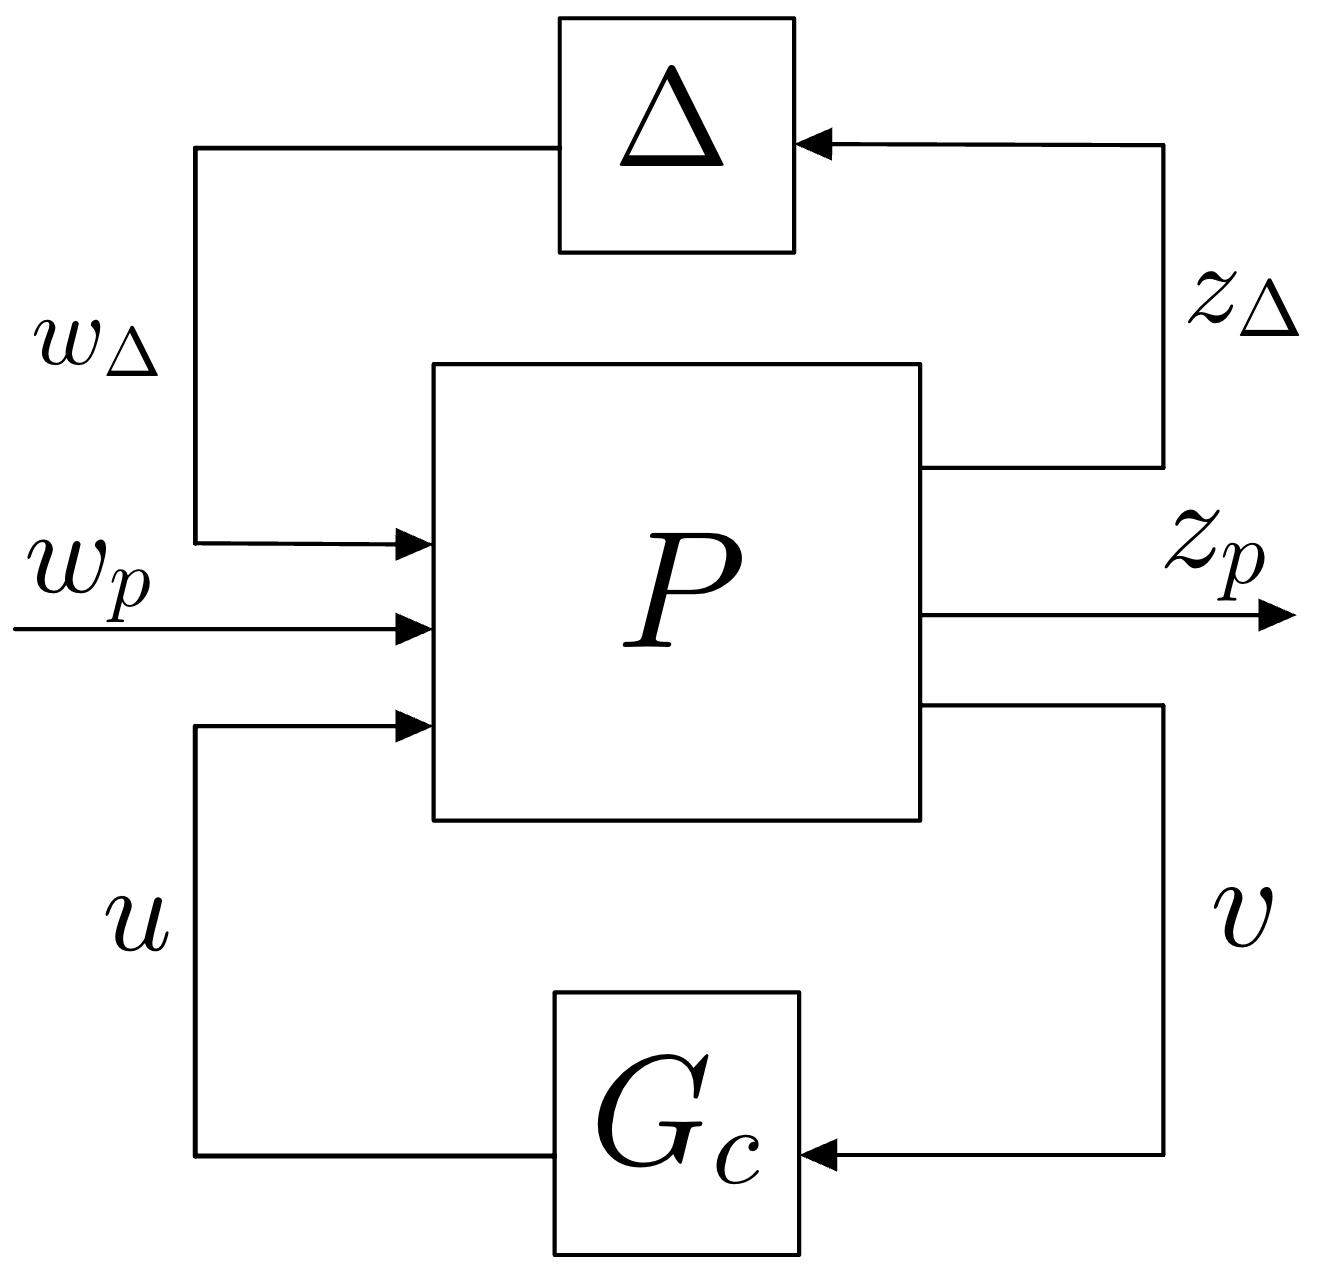
\includegraphics[scale=0.14]{img/pdg.jpg}\\
        $P\Delta{G_c}$ \textsf{general structure}
    \end{center}
    

\noindent
In such a general structure the sources of uncertainty $\Delta_i$ are pulled out to form a \textbf{block diagonal matrix} $\Delta$, that is:
\begin{equation}\label{eq:Delta_blocks}
    \Delta=\text{diag}\{\Delta_i\}=\begin{bmatrix}
        \Delta_1&0&\dots&0\\
        0&\Delta_2&\dots&0\\
        \vdots&\vdots&\ddots&\vdots\\
        0&\dots&0&\Delta_n
    \end{bmatrix}
\end{equation}
We will consider different sources of uncertainty (real, complex full mzatrix, real repeated real scalar values).
\end{multicols}

\subsection{Uncertainty sources}
In the analysis of stability and performances by using the $\mu$-analysis we will consider mainly:
\begin{itemize}
    \itemsep-0.2em
    \item \textbf{Real scalar} perturbations $\Delta_i\in\mathbb{R}$ such that $\vert \Delta_i \vert\le1$; 
    \item \textbf{Complex full matrix} perturbations $\Delta_i(s)\in\mathbb{C}^{m,m}$, $\Vert \Delta_i \Vert_\infty\le1$;
    \item \textbf{Repeated real scalar} perturbations $\Delta_i I_r$, where $I_r$ is an $r\times{r}$ identity matrix, and $\Delta_i\in\mathbb{R}$, $\Delta_i\le{1}$ 
\end{itemize}
In order to perform a computer-aided $\mu$-analysis, how we will see we use the command \texttt{mu} that among all of the parameters, take as input a matrix called \texttt{deltaset}. The main objective of such a matrix is \textit{describing the blocks of \ref{eq:Delta_blocks}}, the block diagonal matrix we mentioned in term of: (i) type, (ii) dimensions, (iii) number of independent locations in which the uncertainty itself appears. By using a summarizing table, we mention the principal pattern we can find in analyzing our feedback control systems. 

\begin{table}[h!]
    \centering
    \begin{tabular}{p{7cm} p{5cm}}
        \toprule[1pt]
        \textbf{Type of $\Delta_i$}&\textbf{\texttt{deltaset} row}\\
        \midrule
        Scalar real parameter&$[-1\quad{1}]$ or $[-1\quad0]$\\
        \midrule
        $f$-repeated real parameter&$[-f\quad{0}]$\\
        \midrule
        Scalar $1\times1$ unmodeled dynamics&$[1\quad{1}]$ or $[1\quad0]$\\
        \midrule
        $r\times{c}$ full unmodeled dynamics&$[r\quad{c}]$\\        \bottomrule[1pt]
    \end{tabular}
    \caption{\texttt{deltaset} for describing $\Delta$}
    \label{tab:deltaset}
\end{table}
\noindent
Wheter in the feedback control system there are $U$ uncertainty sources the final will be such that \texttt{deltaset}$\in\mathbb{R}^{U,2}$.
In the following sections we are going to do some examples which will clarify what is the structure of the \texttt{deltaset} matrix according to the structure of the uncertain plant $G_p(s)$.
The models can be considered for the uncertainty are the following, given the generic parameter $k$: 

\begin{table}[h]
    \centering
    \begin{tabular}{p{8cm} p{6cm}}
        \toprule[1pt]
        \textbf{MODEL SET}&\textbf{Mathematical description}\\
        \midrule
        \textsc{Additive uncertainty set}&$k=k_n+W_k{\Delta_k}, \ \vert \Delta_k \vert \le 1$  \\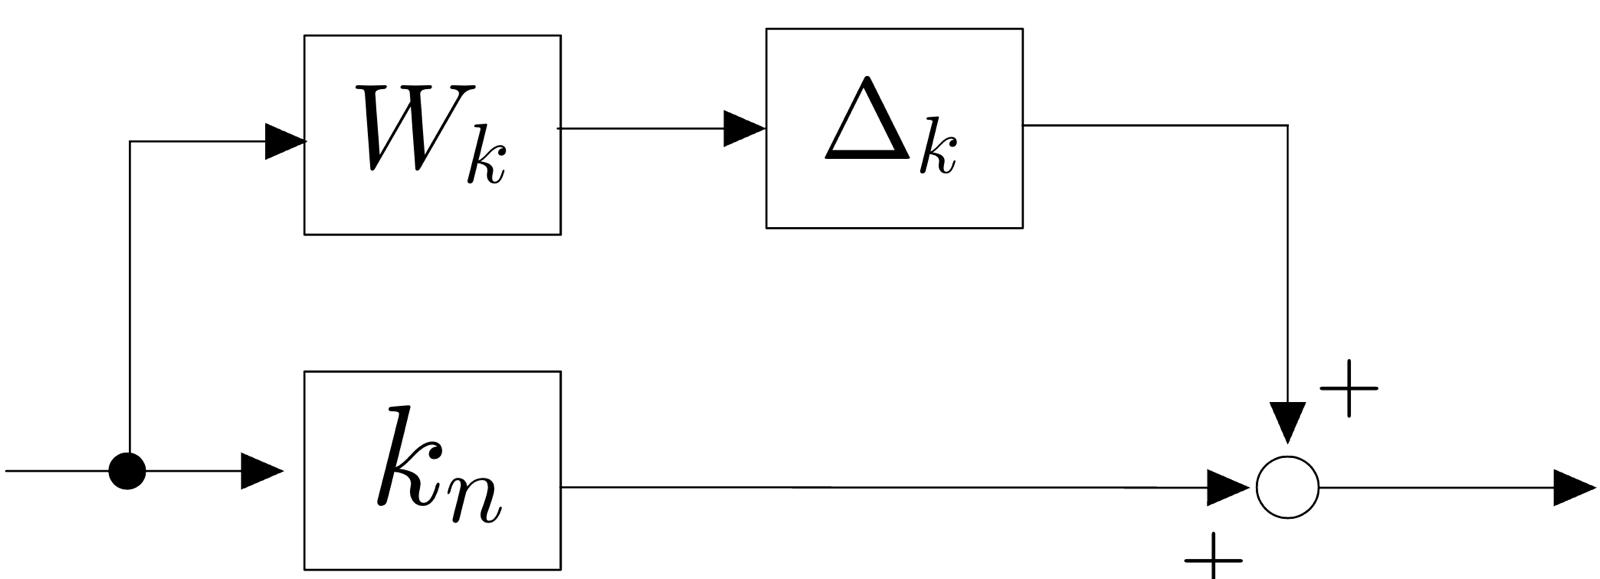
\includegraphics[scale=0.12]{img/add_k.jpg}\\
        \midrule
        \textsc{Multiplicative uncertainty set}&$k=k_n(1+W_k\Delta_k), \ \vert \Delta_k \vert \le1$ \\ 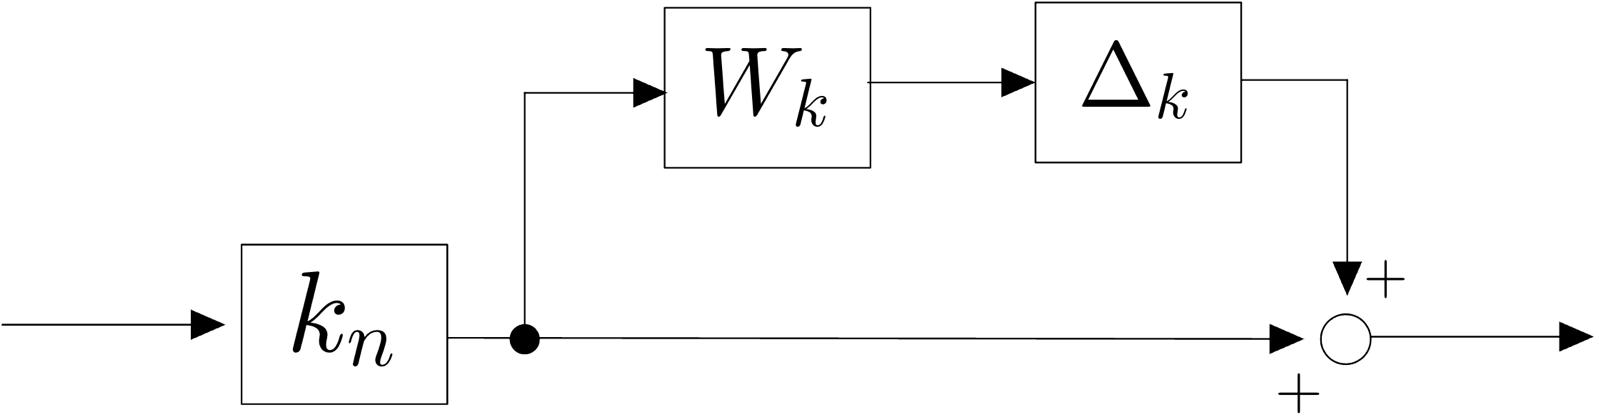
\includegraphics[scale=0.14]{img/mul_k.jpg}\\
        \bottomrule[1pt]
    \end{tabular}
    \caption{Uncertainty model sets}
    \label{tab:uncertainty_set}
\end{table}


\subsection{Fundamental bricks for structured uncertainty}
Going on to analyze the structure of our uncertain system we can find in the transfer function some fundamental bricks that put all together will give us the description through block diagrams of the uncertain plant. \textsf{Some aspects are presented in details for the first example while they are not repeated for the following ones which are using exactly the same steps.}

\subsubsection{Real Pole in \texttt{zpk} form}

\subsubsection*{Example 1 (pole in the feedback path)}
Given the following transfer function for an uncertain plant 
\begin{equation}\label{eq:ex1}
    G_p(s)=\frac{k}{s+p} \quad  
    \underline{k}\le {k} \le \overline{k}, \quad
    \underline{p}\le {p} \le \overline{p}
\end{equation}
we want to obtain its block diagram description. In particular for each parameter is required to obtain the central estimate $k_n$ and $p_n$ and the radius of uncertainty $W_k$ and $W_p$. Compute also the matrix $\Delta$ and the associated \texttt{deltaset} for the command \texttt{mu}.\\
The first step is for computing the value $k_n$, $p_n$, $W_k$ and $W_p$:
\begin{align}
    k_n=\frac{\underline{k}+\overline{k}}{2} \quad
    W_k=\frac{\overline{k}-\underline{k}}{2}, \qquad 
    p_n=\frac{\underline{p}+\overline{p}}{2} \quad
    W_p=\frac{\overline{p}-\underline{p}}{2}
\end{align}
\noindent
At the end of the day, we are likely to build such block diagrams in \textsc{Simulink}\footnote{
    Some algebraic manipulation are needed in order to avoid non proper blocks that -- for sure-- are going to raise an error during the simulation.
}, for this reason we have to manipulate the expression of \Cref{eq:ex1} in order to be able to represent them. If we put in evidence $s$ at the denominator we can write:

\begin{multicols}{2}
    {\large{
        \begin{equation*}
            G_p(s)=\frac{k}{s(1+\frac{p}{s})}=k \frac{\frac{1}{s}}{1+\frac{p}{s}}
        \end{equation*}
    }}
    The first term of the expression is simply a gain, while we can see the second term as a \textit{feedback configuration} with negative feedback.
    \newcolumn 
    \begin{center}
        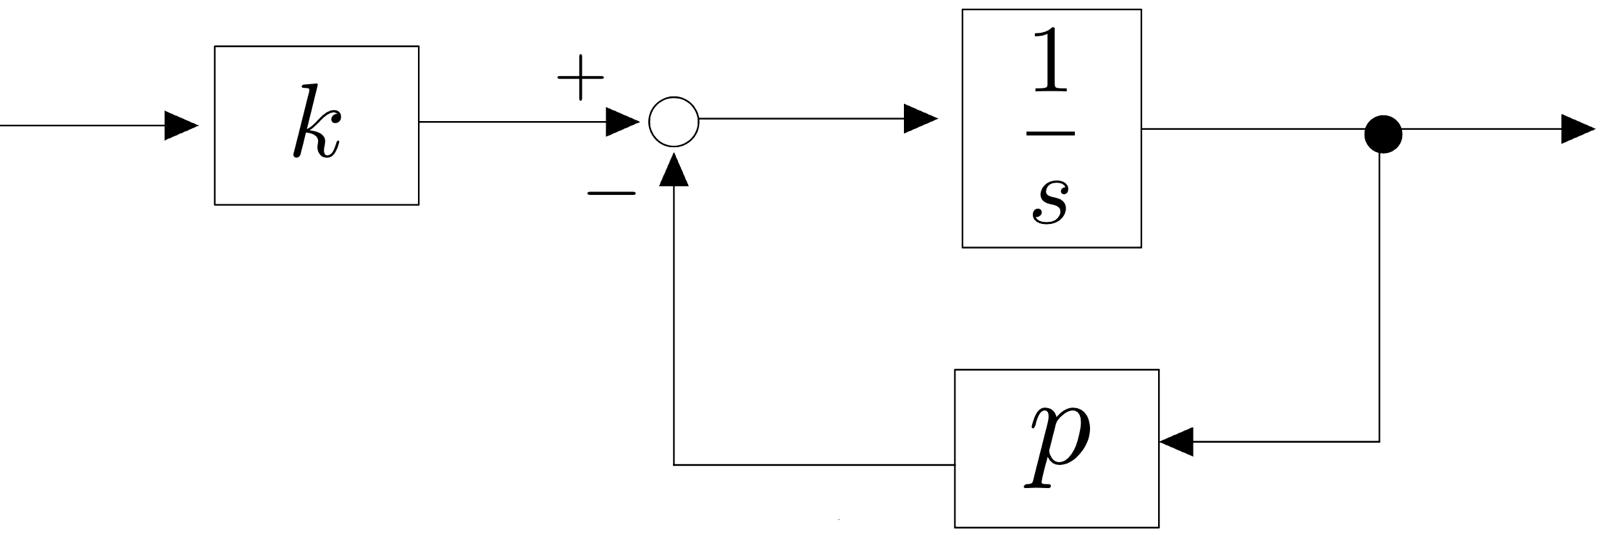
\includegraphics[scale=0.15]{img/ex1.jpg}\\
        \textsf{Block diagram for \Cref{eq:ex1}}
    \end{center}
\end{multicols}

\noindent
\textsf{\large \textbf{Additive Uncertainty Set}}\\
If we use the as uncertainty set the \textit{additive one} the block diagram we have showed changes as follows: 

\begin{figure}[h]
    \centering
    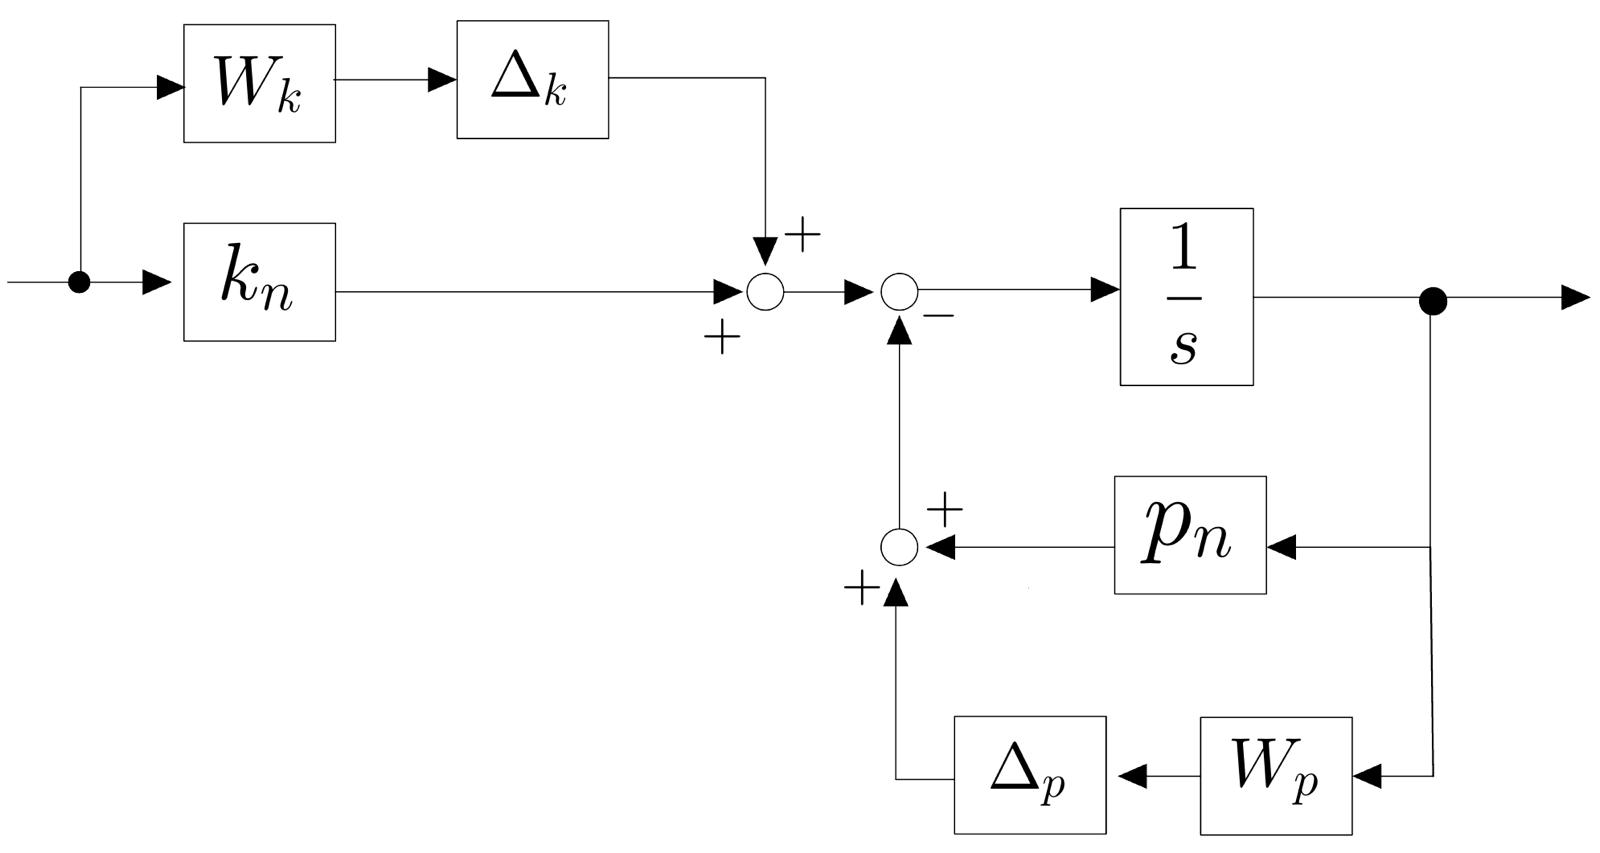
\includegraphics[scale=0.23]{img/ex1_add.jpg}
    \caption{Block diagram of $G_p(s)$ (additive model)}
\end{figure}
\noindent
Note that we have only added the for the parameters the uncertain description as indicated in \Cref{tab:uncertainty_set}. With the objective of obtaining the the $P\Delta{G_c}$ structure we have to: (i) put such a diagram in the Feedback control System (FCS) scheme; (ii) pull out all of the $\Delta_i$ blocks; (iii) pull out the controller $G_c$. \\
More interesting is the construction of the matrix $\Delta$ and its describing matrix \texttt{deltaset}. For this aim is crucial that all of the uncertainty channels are properly numbered. The block diagram becomes the one in \Cref{fig:ex1_num}, where there are also the signals entering/coming from the (structured) uncertainty block $\Delta$. According to the numbering we use in the block diagram we have to insert the diagonal blocks into $\Delta$ as reported here:

\begin{equation}
    \Delta=\begin{bmatrix}
        {\color{red}{\Delta_k}}&0\\
        0&{\color{blue}{\Delta_p}}
    \end{bmatrix} \qquad
    \texttt{deltaset}=[
        \underbrace{\texttt{{\color{red}{-1,1}}}}_{\color{red}1}; 
        \underbrace{\texttt{{\color{blue}-1,1}}}_{\color{blue}2}]
\end{equation}

\begin{figure}[h]
    \centering
    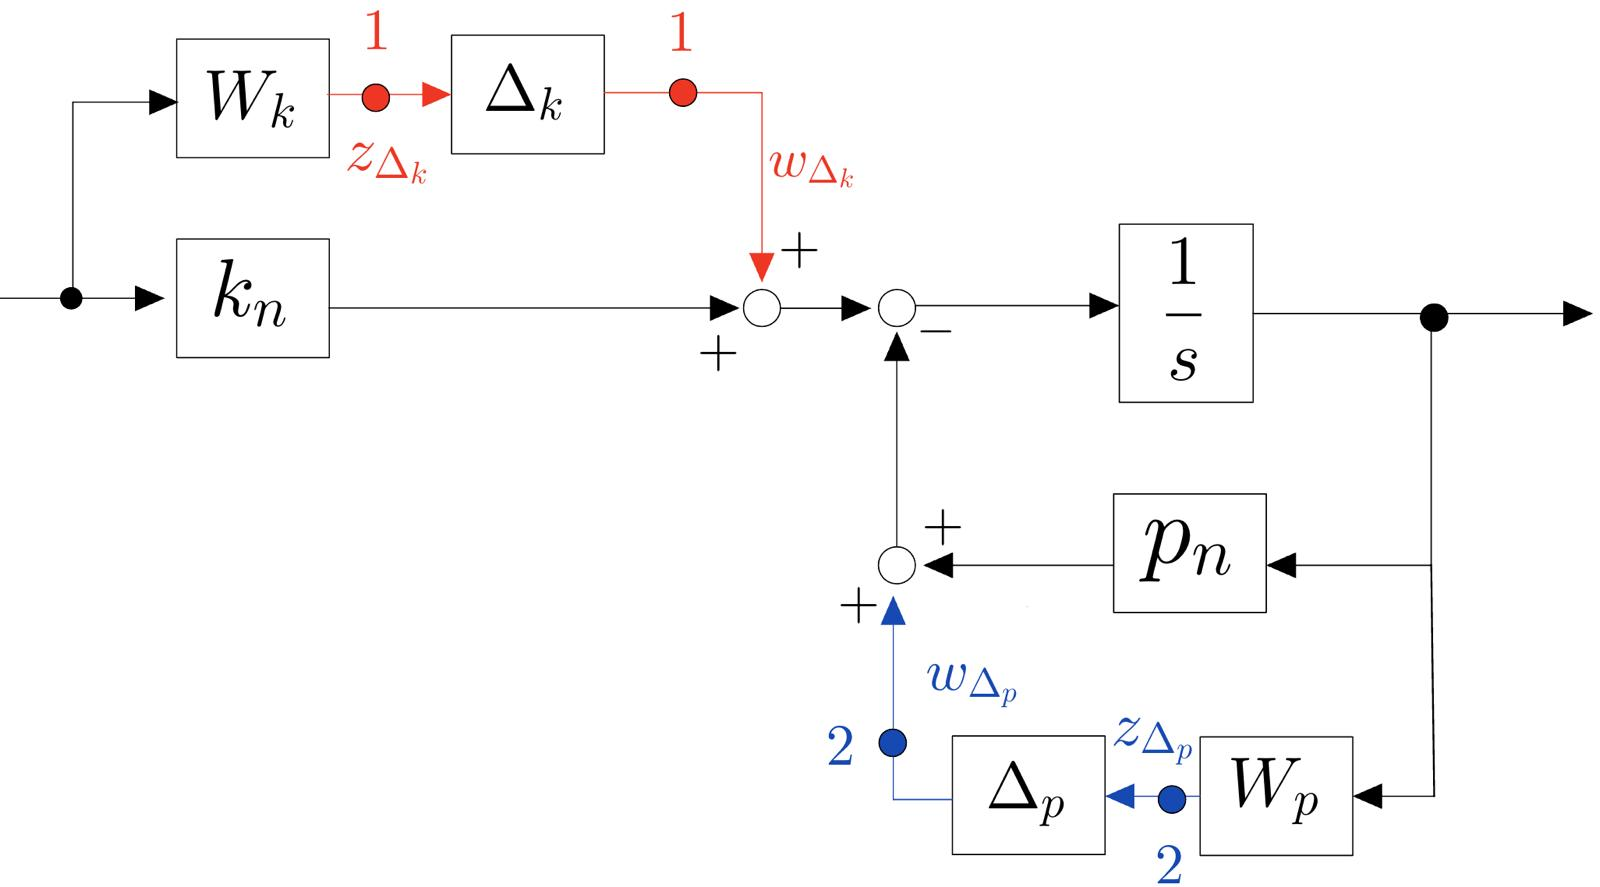
\includegraphics[scale=0.23]{img/ex1_num.jpg}
    \caption{Block diagram of $G_p(s)$ (additive) with numbered sources}
    \label{fig:ex1_num}
\end{figure}


\noindent
The first block of $\Delta$ is the one related to the uncertain parameter $\color{red} k$, the second the one related to the uncertain parameter $\color{blue} p$. Let the colors guide you in the understanding the relationship existing between the block diagram and related $\Delta$ and \texttt{deltaset}.\\

\noindent
\textsf{\large \textbf{Multiplicative Uncertainty Set}}\\
Identical reasoning can be done, if we assume to take as model of uncertainty the \textit{multiplicative one}. Substituting in the general scheme, the structure for the uncertain parameters from the \Cref{tab:uncertainty_set}, the scheme in \Cref{fig:ex1_mul} is obtained. The associated matrix $\Delta$ and the \texttt{deltaset} array are the same as before.

\begin{figure}[h]
    \centering
    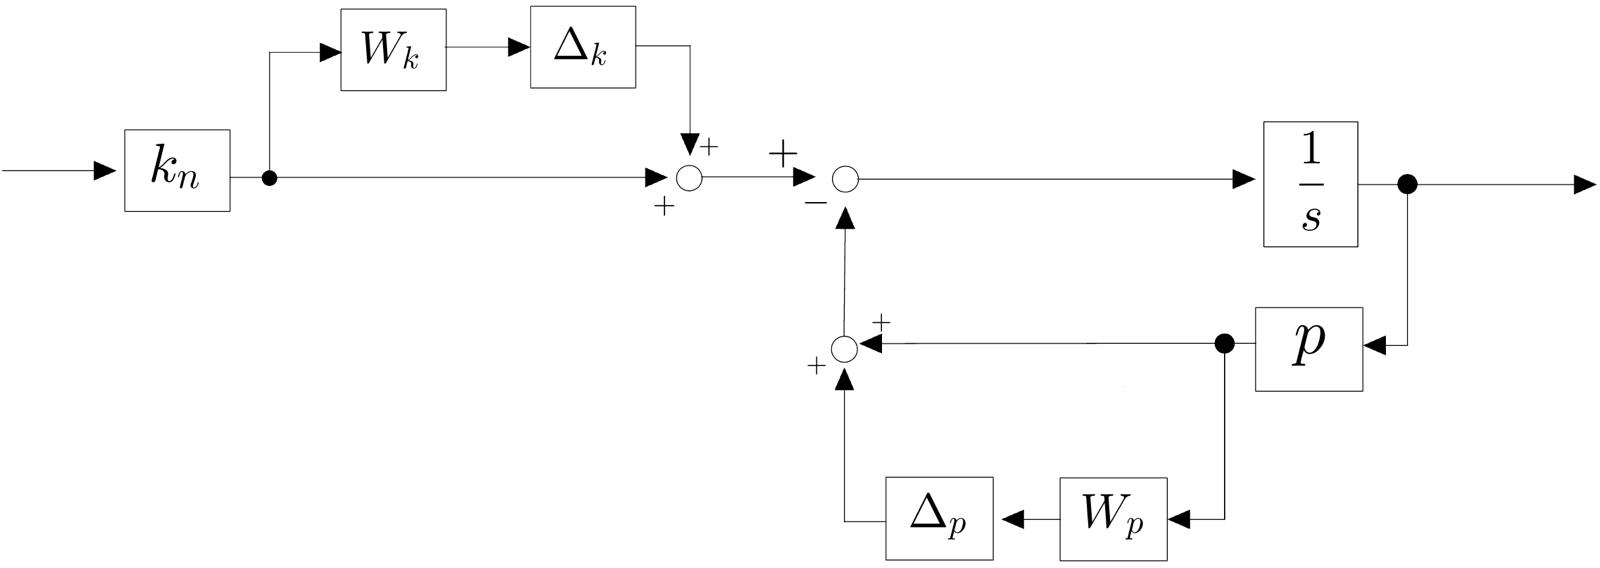
\includegraphics[scale=0.27]{img/ex1_mul.jpg}
    \caption{Block diagram for $G_p(s)$ (multiplicative set)}
    \label{fig:ex1_mul}
\end{figure}

\begin{figure}
    \centering
    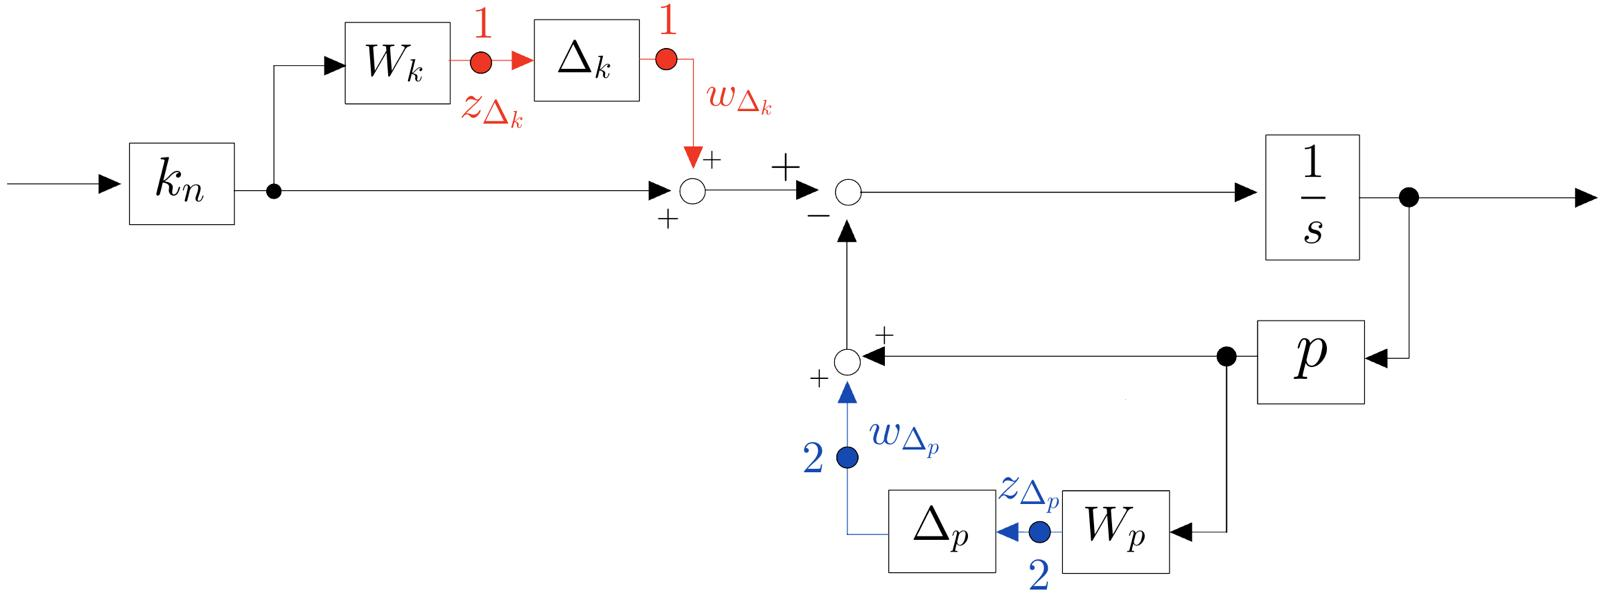
\includegraphics[scale=0.3]{img/ex2_num.jpg}
    \caption{Block diagram for $G_p(s)$ (multiplicative set) with numbered uncertainty channels}
\end{figure}

\newpage
\subsubsection*{Example 2 (model the reciprocal of an uncertain parameter)}
Given the following plant
\begin{equation}
    G_p(s)=\frac{k}{1+s\tau}, \quad     
\end{equation}
is required to find a block diagram description of it, in a way that can be implemented in a simulink scheme. 
\begin{multicols}{2}
    \noindent
    A rearragement of the terms is needed: 
\begin{equation}
    G_p(s)=k \ \frac{\frac{1}{s}\cdot \frac{1}{\tau}}{1+\frac{1}{s\tau}}
\end{equation}
We omit the gain, to focus our attention on the second part of the transfer function.

\newcolumn
The second term can be represented as:
\begin{center}
    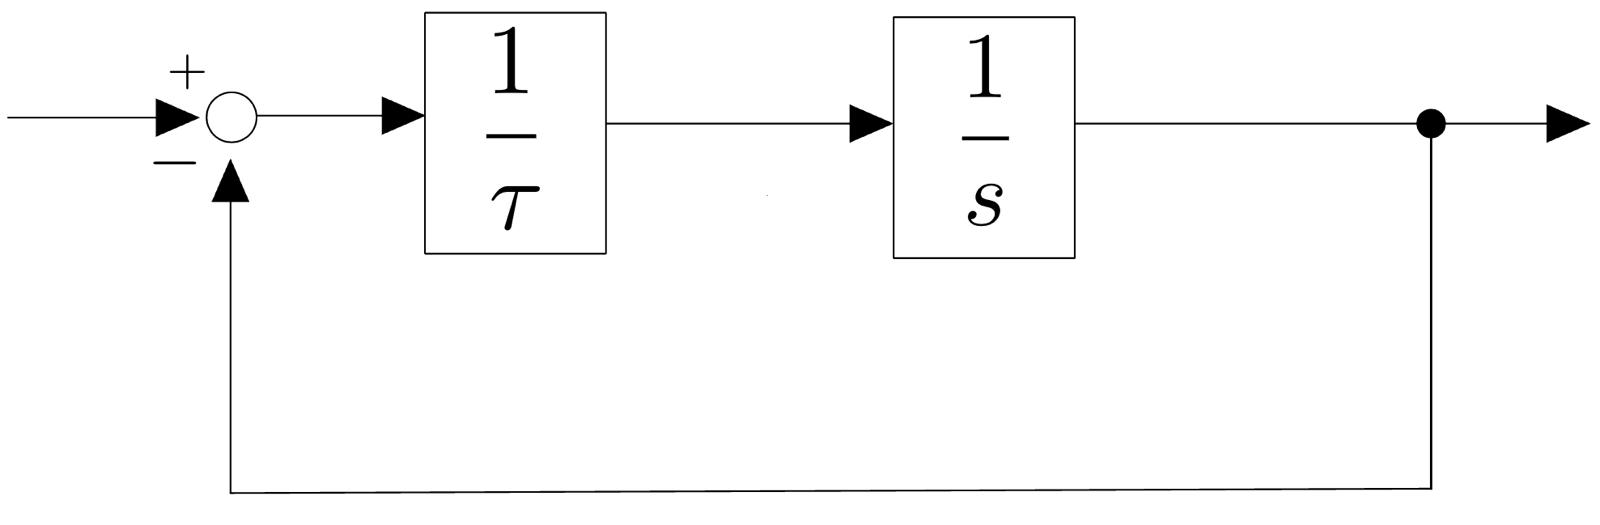
\includegraphics[scale=0.13]{img/tau.jpg}
\end{center}
\end{multicols}


\noindent
The second term can be recasted in a basic feedback structure whose direct path has the block $1/{s\tau}$, simply 1 in the feedback path. But how can we draw the diagram for the inverse of the uncertain parameter? It depends from the type of uncertainty set. 

\begin{multicols}{2}
    \noindent
\textbf{\textsf{Multiplicative set}}\\
The term $1/\tau$ can be written as:
\begin{equation}
    \frac{1}{\tau}=\frac{1}{\tau_n}\cdot
    \frac{1}{1+W_\tau \Delta_\tau}
\end{equation}
The related block diagram representation is:
\begin{center}
    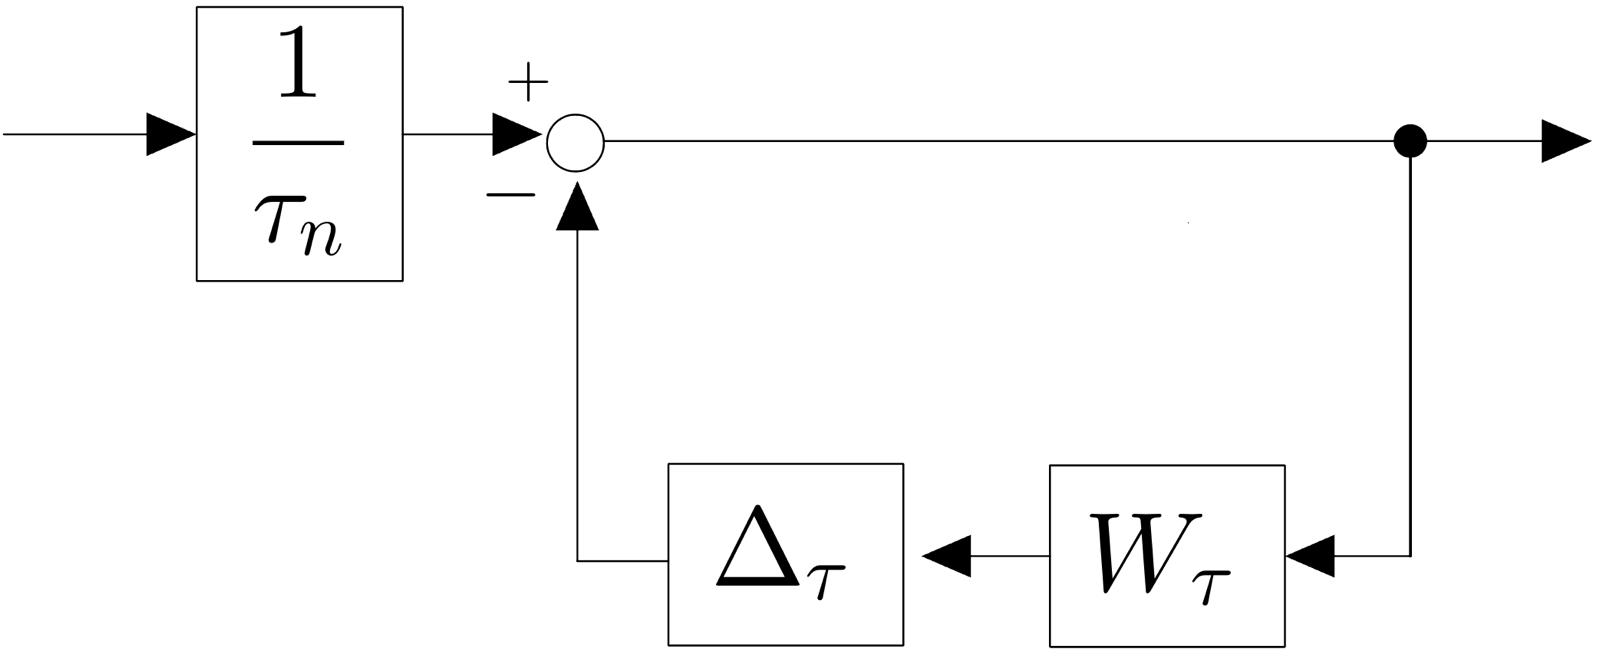
\includegraphics[scale=0.13]{img/tau_mul.jpg}
\end{center}

\newcolumn
\noindent
\textbf{\textsf{Additive set}}\\
The term $1/\tau$ can be written as:
\begin{equation}
    \frac{1}{\tau}=\frac{1}{\tau_n+W_\tau \Delta_\tau}=
    \frac{\frac{1}{\tau_n}}{1+\frac{W_\tau \Delta_\tau}{\tau_n}}
\end{equation}
The related block diagram representation is:
\begin{center}
    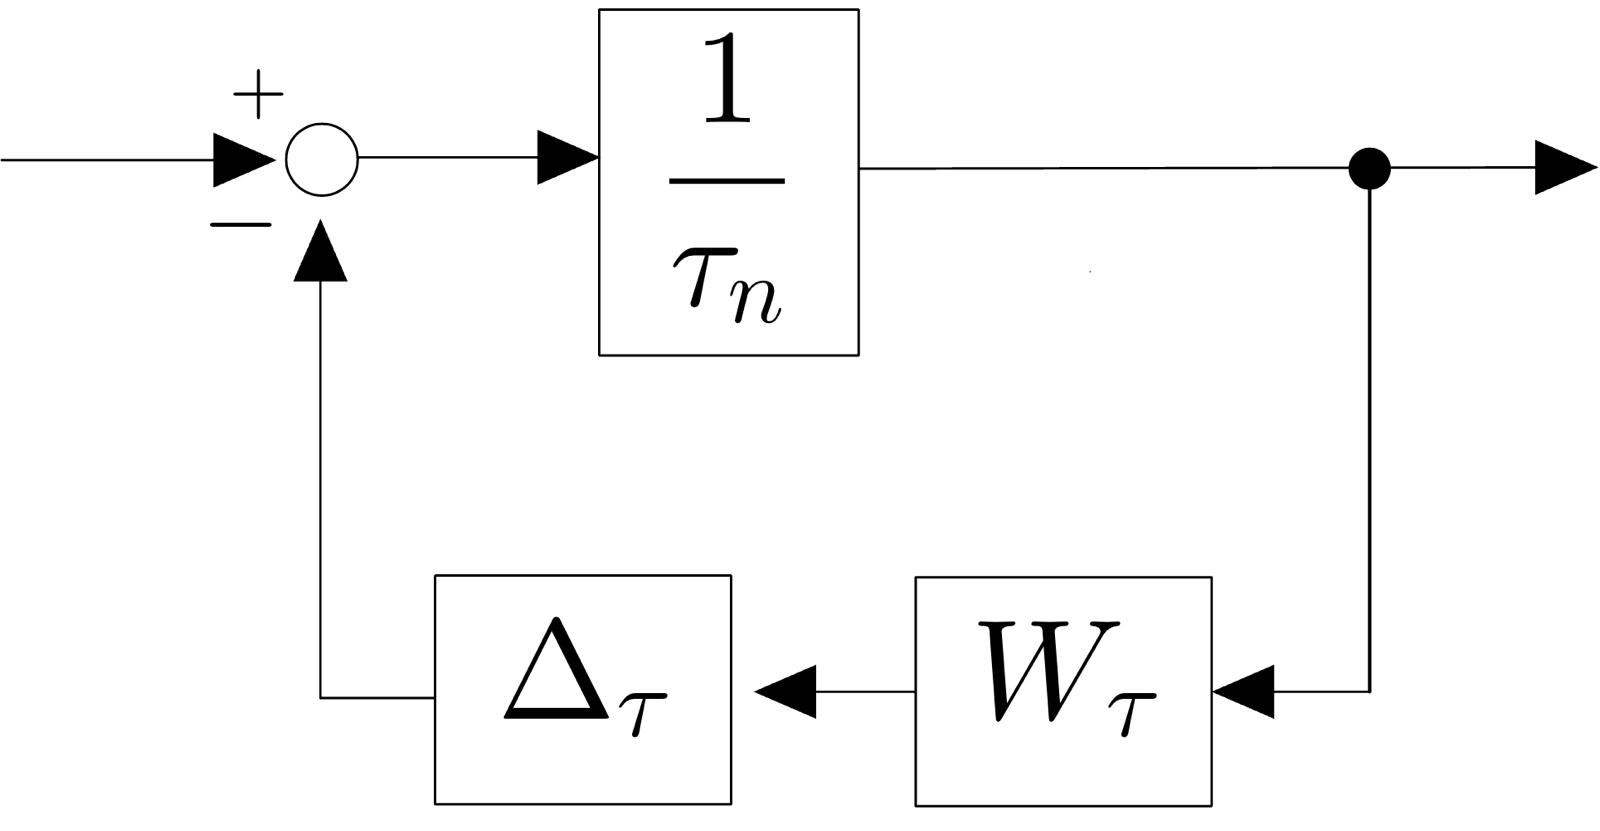
\includegraphics[scale=0.11]{img/tau_add.jpg}
\end{center}
\end{multicols}
\noindent
The remaining part of the discussion, about the port numbering and block $\Delta$ description, the way we retrieve $\Delta_\tau$ and $W_\tau$ does not change. This is the reason why we omit this part.
 
\subsubsection{Real pole in DC-gain form}
Here the objective is to analyze the block diagrams for the uncertain plant described by the following transfer function in \textit{DC-gain (or time constant) form}:
\begin{equation}\label{eq:ex2}
    G_p(s)=\frac{k}{1+\frac{s}{p}} \qquad
    \underline{k}\le {k} \le \overline{k}, \quad
    \underline{p}\le {p} \le \overline{p}
\end{equation}
\noindent

\begin{multicols}{2}
    \noindent
    Following the same path we algebrically manipulate the \Cref{eq:ex2} in order to obtain:
    \begin{equation*}
        G_p(s)=k \ \frac{\frac{p}{s}}{1+\frac{p}{s}}
    \end{equation*}
    \newcolumn
    \begin{center}
        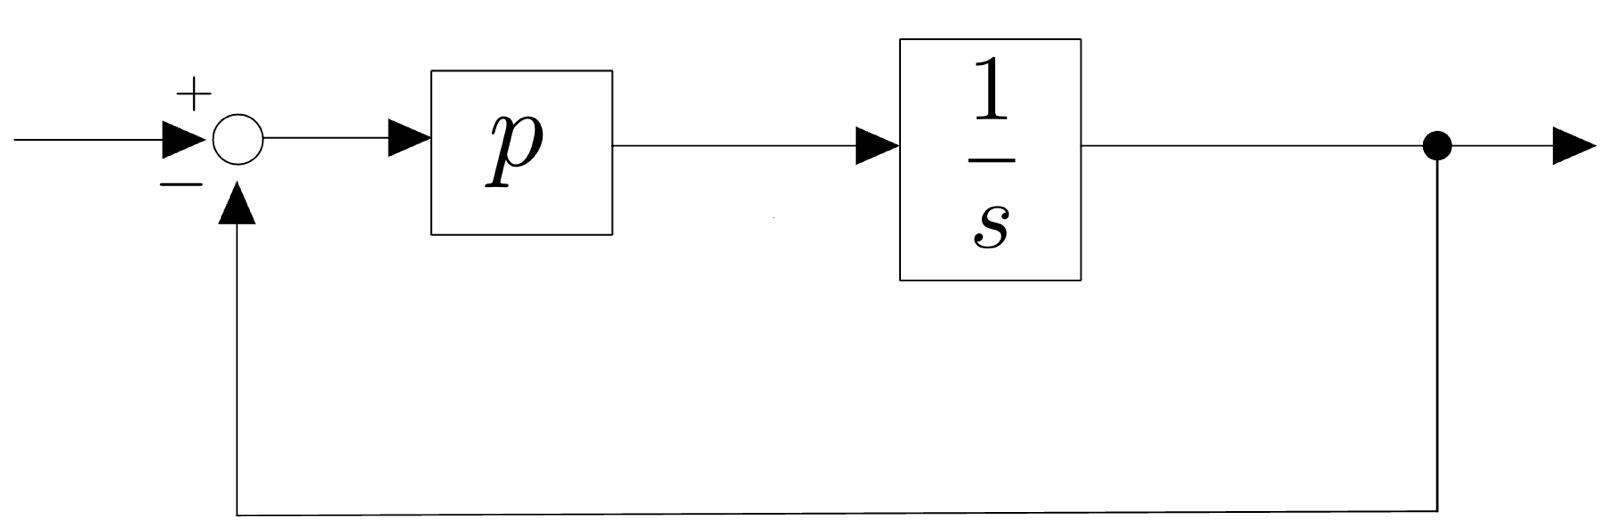
\includegraphics[scale=0.15]{img/ex2.jpg}
    \end{center}
\end{multicols}
\noindent
No other comments are needed  for modeling $p$ since it is a simple uncertain parameter whose modeling can follow the \Cref{tab:uncertainty_set}.


\subsubsection{Complex conjugate poles}

\end{document}